\documentclass[11pt]{article}

\usepackage{fix-cm}
\usepackage{tikz}
\usetikzlibrary{shapes,backgrounds,calc,patterns}
\usepackage{amsmath,amsthm} 
\usepackage{amssymb}
\usepackage[framemethod=tikz]{mdframed}
\usepackage{draculatheme}
\usepackage{mathrsfs}
\usepackage{changepage}
\usepackage{multicol}
\usepackage{mathtools}
\usepackage{hyperref}
\usepackage{slashed}
\usepackage{enumerate}
\usepackage{booktabs}
\usepackage{enumitem}
\usepackage{kantlipsum} 
\usepackage{tabularx}
\usepackage{array}
\usepackage{makecell}
\usepackage{pgfplots}
\pgfplotsset{compat=1.18}
\usetikzlibrary{decorations.markings}

\setlength{\parindent}{0pt}

\newmdenv[
  topline=false,
  bottomline=true,
  rightline=false,
  leftline=true,
  linewidth=1.5pt,
  linecolor=black, % default color, will be overridden in custom commands
  backgroundcolor=draculabg, % Needed for Dracula theme
  fontcolor=draculafg, % Needed for Dracula theme
  innertopmargin=0pt,
  innerbottommargin=5pt,
  innerrightmargin=10pt,
  innerleftmargin=10pt,
  leftmargin=0pt,
  rightmargin=0pt,
  skipabove=\topsep,
  skipbelow=\topsep,
]{customframedproof}

\newenvironment{proofpart}[2][black]{
    \begin{mdframed}[
        topline=false,
        bottomline=false,
        rightline=false,
        leftline=true,
        linewidth=1pt,
        linecolor=#1!40, % Custom color
        % innertopmargin=10pt,
        % innerbottommargin=10pt,
        innerleftmargin=10pt,
        innerrightmargin=10pt,
        leftmargin=0pt,
        rightmargin=0pt,
        % skipabove=\topsep,
        % skipbelow=\topsep%
    ]
    \noindent
    \begin{minipage}[t]{0.08\textwidth}%
        \textbf{#2}%
    \end{minipage}%
    \begin{minipage}[t]{0.90\textwidth}%
        \begin{adjustwidth}{0pt}{0pt}%
}{
    \end{adjustwidth}
    \end{minipage}
    \end{mdframed}
}

\newenvironment{solution}
  {\textit{Solution.}}



%%% AESTHETICS %%%
%-%-%-%-%-%-%-%-%-%-%-%-%-%-%-%-%-%-%-%-%-%-%-%-%-%-%-%-%-%-%-%-%-%-%-%-%-%-%


%%% Dimensions and Spacing %%%
\usepackage[left=0.5in,right=0.5in,top=1in,bottom=1in]{geometry}
% \usepackage{setspace}
% \linespread{1}
\usepackage{listings}

%%% Define new colors %%%
\usepackage{xcolor}
\definecolor{orangehdx}{rgb}{0.96, 0.51, 0.16}

% Normal colors
\definecolor{xred}{HTML}{BD4242}
\definecolor{xblue}{HTML}{4268BD}
\definecolor{xgreen}{HTML}{52B256}
\definecolor{xpurple}{HTML}{7F52B2}
\definecolor{xorange}{HTML}{FD9337}
\definecolor{xdotted}{HTML}{999999}
\definecolor{xgray}{HTML}{777777}
\definecolor{xcyan}{HTML}{80F5DC}
\definecolor{xpink}{HTML}{F690EA}
\definecolor{xgrayblue}{HTML}{49B095}
\definecolor{xgraycyan}{HTML}{5AA1B9}

% Dark colors
\colorlet{xdarkred}{red!85!black}
\colorlet{xdarkblue}{xblue!85!black}
\colorlet{xdarkgreen}{xgreen!85!black}
\colorlet{xdarkpurple}{xpurple!85!black}
\colorlet{xdarkorange}{xorange!85!black}
\definecolor{xdarkcyan}{HTML}{008B8B}
\colorlet{xdarkgray}{xgray!85!black}

% Very dark colors
\colorlet{xverydarkblue}{xblue!50!black}

% Document-specific colors
\colorlet{normaltextcolor}{black}
\colorlet{figtextcolor}{xblue}

% Enumerated colors
\colorlet{xcol0}{black}
\colorlet{xcol1}{xred}
\colorlet{xcol2}{xblue}
\colorlet{xcol3}{xgreen}
\colorlet{xcol4}{xpurple}
\colorlet{xcol5}{xorange}
\colorlet{xcol6}{xcyan}
\colorlet{xcol7}{xpink!75!black}

% Blue-Purple (should just used colorbrewer...)
\definecolor{xrainbow0}{HTML}{e41a1c}
\definecolor{xrainbow1}{HTML}{a24057}
\definecolor{xrainbow2}{HTML}{606692}
\definecolor{xrainbow3}{HTML}{3a85a8}
\definecolor{xrainbow4}{HTML}{42977e}
\definecolor{xrainbow5}{HTML}{4aaa54}
\definecolor{xrainbow6}{HTML}{629363}
\definecolor{xrainbow7}{HTML}{7e6e85}
\definecolor{xrainbow8}{HTML}{9c509b}
\definecolor{xrainbow9}{HTML}{c4625d}
\definecolor{xrainbow10}{HTML}{eb751f}
\definecolor{xrainbow11}{HTML}{ff9709}

%%% FIGURES %%%
\usepackage{graphicx}  
% \graphicspath{ {images/} }  
% \numberwithin{figure}{section}
\usepackage{float}
\usepackage{caption}

%%% Hyperlinks %%%
\usepackage{hyperref}
\definecolor{horange}{HTML}{f58026}
\hypersetup{
	colorlinks=true,
	linkcolor=horange,
	filecolor=horange,      
	urlcolor=horange,
}

\newcommand{\mysqrt}[1]{%
  \mathpalette\foo{#1}%
}
\newcommand{\dmysqrt}[1]{%
  \mathpalette\foodisplay{#1}%
}

\newcommand{\sol}[1]{
    \begin{customframedproof}[linecolor=orangehdx!75,]
        \begin{solution}
        #1
        \end{solution}
    \end{customframedproof}
}

% !TeX spellcheck = off
\newcommand{\foo}[2]{%
  % #1: math style, #2: content
  \sbox0{$#1\sqrt{#2}$}% Measure the size of the standard sqrt in the current style
  \begin{tikzpicture}[baseline=(sqrt.base)]
    \node[inner sep=0, outer sep=0] (sqrt) {$#1\sqrt{#2}$}; % Use the current math style
    \draw([yshift=-0.045em]sqrt.north east) -- ++(0,-0.5ex); % Draw the tick
  \end{tikzpicture}%
}
% !TeX spellcheck = off
\newcommand{\foodisplay}[2]{%
  % #1: math style, #2: content
  \sbox0{$#1\sqrt{#2}$}% Measure the size of the standard sqrt in the current style
  \begin{tikzpicture}[baseline=(sqrt.base)]
    \node[inner sep=0, outer sep=0] (sqrt) {$\displaystyle\sqrt{#2}$}; % Force displaystyle
    \draw[line width=0.4pt] ([yshift=-0.044em]sqrt.north east) -- ++(0,-0.5ex); % Draw the tick
  \end{tikzpicture}%
}

\newcommand{\barNotationT}[1]{\bigg|_{t = #1}}

\newcommand{\cyanit}[1]{\textit{\textcolor{cyan}{#1}}}

\newcommand{\brackett}[1]{\left\langle #1 \right\rangle}

\newcommand{\norm}[1]{\left\lVert \mathbf{#1}\right\rVert}

\newcommand{\imb}{\mb{i}}
\newcommand{\jmb}{\mb{j}}
\newcommand{\kmb}{\mb{k}}
\newcommand{\rmb}{\mb{r}}
\newcommand{\umb}{\mb{u}}

\newcommand{\vecfuc}[2]{\mb{#1}(#2)}
\newcommand{\dvecfuc}[2]{\mb{#1}'(#2)}
\newcommand{\normdvecfuc}[2]{||\mb{#1}'(#2)||}

\newcommand{\proj}{\text{proj}}

\newcommand{\mb}[1]{\mathbf{#1}}

% \renewcommand{\theenumi}{\arabic{enumi}} 
% \renewcommand{\labelenumi}{\theenumi.}

\title{Multivariable Calculus Practice Set III}
\author{Paul Beggs}
\date{\today}

%%% Custom Comands %%%
% Natural Numbers 
\newcommand{\N}{\ensuremath{\mathbb{N}}}

% Whole Numbers
\newcommand{\W}{\ensuremath{\mathbb{W}}}

% Integers
\newcommand{\Z}{\ensuremath{\mathbb{Z}}}

% Rational Numbers
\newcommand{\Q}{\ensuremath{\mathbb{Q}}}

% Real Numbers
\newcommand{\R}{\ensuremath{\mathbb{R}}}

% Complex Numbers
\newcommand{\C}{\ensuremath{\mathbb{C}}}

\newcommand{\I}{\ensuremath{\mathbb{I}}}

\newcommand{\p}{\partial}

\begin{document}

\maketitle

\begin{enumerate}
  \item (3 points) Determine the absolute extrema for the function \(f(x,y) = x^{2} + 3y^{2} - 2x - y - xy\) on the triangular region with vertices \((0,0)\), \((2,0)\), and \((0,1)\). \\
        \sol{
          We first find the critical points of the function:
          \begin{align*}
            \nabla f(x,y) & = \langle 2x - 2 - y, \, 6y - 1 - x \rangle = \mathbf{0}  \\
            \implies y    & = 2x - 2 \quad \text{and} \quad x = 6(2x - 2) - 1 - x     \\
            \implies y    & = \tfrac{4}{11} \quad \text{and} \quad x = \tfrac{13}{11}
          \end{align*}
          This gives the critical point \(\boxed{\left(\frac{13}{11}, \frac{4}{11}\right)}\). We also need to check the boundary of the region. Thus:
          \begin{enumerate}[label=(\(\ell_{\arabic*}\)):]
            \item \(y = 0, \, 0 \leq x \leq 2 \implies f(x,y) = g(x) = x^{2} + 3(0)^{2} - 2x - (0) - x(0) = x^{2} - 2x \implies g'(x) = 2x - 2\). Therefore, the critical points are \(\boxed{(1,0)}\). \\
            \item \(x = 0, \, 0 \leq y \leq 1 \implies f(x,y) = h(y) = (0)^{2} + 3y^{2} - (0) - y - 0 = 3y^{2} - y \implies h'(y) = 6y - 1\). Hence, the critical points are \(\boxed{\left(0, \frac{1}{6}\right)}\). \\
            \item  \(y = 1 - \tfrac{1}{2}x, \, 0 \leq x \leq 2 \implies f(x,y) = k(x) = x^{2} + 3\left(1 - \tfrac{1}{2}x\right)^{2} - 2x - \left(1 -\tfrac{1}{2}x\right) - x\left(1 - \frac{1}{2}x\right).\)
                  Solving this equation for \(x\):
                  \begin{align*}
                    k(x)           & = x^{2} + 3\left(1 - \tfrac{1}{2}x - \tfrac{1}{2}x + \tfrac{1}{4}x^{2}\right) - 2x - 1 + \tfrac{1}{2}x - x + \tfrac{1}{2}x^{2} \\
                                   & = x^{2} + 3\left(1 - x + \tfrac{1}{4}x^{2}\right) - 2x - 1 + \tfrac{1}{2}x - x + \tfrac{1}{2}x^{2}                             \\
                                   & = \left[x^{2} + \tfrac{3}{4}x^{2} + \tfrac{1}{2}x^{2}\right] + \left[-3x - 2x - \tfrac{1}{2}x\right] + \left[3 - 1\right]      \\
                                   & = \tfrac{9}{4}x^{2} - \tfrac{7}{2}x + 2                                                                                        \\
                                   & = \tfrac{1}{4}(9x^{2} - 22x + 8)                                                                                               \\
                    \implies k'(x) & = \tfrac{1}{4} \cdot \tfrac{d}{dx}[9x^{2} - 22x + 8]                                                                           \\
                    0              & = \tfrac{1}{2}(9x - 11)                                                                                                        \\
                    x              & = \tfrac{11}{9}
                  \end{align*}
                  Using this \(x\)-value, we plug it back into our equation for \(y\) to get the critical point \(\boxed{\left(\frac{11}{9}, \frac{7}{18}\right)}\).
          \end{enumerate}
          With our function's and lines' critical points found, we also need to find the vertices of the triangle:
          \begin{align*}
            f(0,0) & = 0^{2} + 3(0)^{2} - 2(0) - 0 - 0(0) = 0 \\
            f(2,0) & = 2^{2} + 3(0)^{2} - 2(2) - 0 - 2(0) = 0 \\
            f(0,1) & = 0^{2} + 3(1)^{2} - 2(0) - 1 - 0(1) = 2
          \end{align*}          
          Now that we have our critical points, we can evaluate the function at each of these points to determine the absolute extrema:
          \begin{align*}
            f\left(\tfrac{13}{11}, \tfrac{4}{11}\right) & = \left(\tfrac{13}{11}\right)^{2} + 3\left(\tfrac{4}{11}\right)^{2} - 2\left(\tfrac{13}{11}\right) - \tfrac{4}{11} - \tfrac{13}{11} \\
            &\approx -1.363\ldots \\
            f(1,0) & = 1^{2} + 3(0)^{2} - 2(1) - 0 - 1(0) \\
            &= -1 \\
            f\left(0, \tfrac{1}{6}\right)              & = 0^{2} + 3\left(\tfrac{1}{6}\right)^{2} - 2(0) - \tfrac{1}{6} - 0\\
            &\approx -0.083\ldots \\
            f\left(\tfrac{11}{9}, \tfrac{7}{18}\right)  & = \left(\tfrac{11}{9}\right)^{2} + 3\left(\tfrac{7}{18}\right)^{2} - 2\left(\tfrac{11}{9}\right) - \tfrac{7}{18} - \tfrac{11}{9} \\
            &\approx -1.361\ldots
          \end{align*}
          Thus, this gives us 7 critical points:
          \begin{multicols}{2}
            \begin{center}
            \begin{tabular}{ccc}
              \toprule
              \textbf{Point} & \(f(x,y)\) & \textbf{Type} \\ \midrule
              \(\left(\tfrac{13}{11}, \tfrac{4}{11}\right)\) & \(-1.364\) & Interior CP \\ \midrule
              \((1,0)\) & \(-1\) & \(\ell_{1}\) \\ \midrule
              \(\left(0, \tfrac{1}{6}\right)\) & \(-0.083\) & \(\ell_{2}\) \\ \midrule
              \(\left(\tfrac{11}{9}, \tfrac{7}{18}\right)\) & \(-1.361\) & \(\ell_{3}\) \\ \midrule
              \((0,0)\) & \(0\) & Vertex 1 \\ \midrule
              \((2,0)\) & \(-2\) & Vertex 2 \\ \midrule
              \((0,1)\) & \(2\) & Vertex 3 \\ \bottomrule
            \end{tabular}
            \end{center}

            \flushright
            \begin{tikzpicture}[scale=2.45]
              \draw[->] (-0.5,0) -- (2.5,0) node[right] {\(x\)};
              \draw[->] (0,-0.5) -- (0,1.5) node[above] {\(y\)};
              \draw[color=horange, thick] (0,0) -- (2,0) -- (0,1) -- cycle;
              \node[below left] at (0,0) {\(0\)};
              \node[below] at (2,0) {\(2\)};
              \node[left] at (0,1) {\(1\)};
              \node[below] at (1,0) {\(\ell_{1}\)};
              \node[left] at (0,0.5) {\(\ell_{2}\)};
              \node[below] at (1,0.8) {\(\ell_{3}\)};
              \node[scale=0.7] at (13/11, 4/11) {\(\bullet\)};
              \node[scale=0.7] at (11/9, 7/18) {\(\bullet\)};
              \node[scale=0.7] at (0,1) {\(\bullet\)};
              \node[scale=0.7] at (0,0) {\(\bullet\)};
              \node[scale=0.7] at (2,0) {\(\bullet\)};
              \node[scale=0.7] at (0,1/6) {\(\bullet\)};
            \end{tikzpicture}
          \end{multicols}
          With these values, we can see that the absolute maximum is \(\boxed{2}\), which occurs at the vertex \((0,1)\), and the absolute minimum is \(\boxed{-1.364}\), which occurs at the critical point \(\left(\tfrac{13}{11}, \tfrac{4}{11}\right)\).

        }

        \textit{Note that the points that I labeled as critical points should just be labeled as points. The critical points are the ones that are in the interior of the region.}
\newpage
  \item (1 point each) Convert each as indicated; leave each answer as exact:
        \begin{enumerate}
          \item Convert the rectangular point \((-5,1)\) to polar coordinates. \\
          \sol{
            \begin{align*}
              r & = \mysqrt{(-5)^{2} + 1^{2}} = \mysqrt{26} \\
              \theta & = \arctan\left(\tfrac{1}{-5}\right) = \arctan\left(-\tfrac{1}{5}\right) = \tfrac{7\pi}{6}
            \end{align*}
            The polar coordinates are \(\boxed{\left(\mysqrt{26}, \tfrac{7\pi}{6}\right)}\).
          }
          \item Convert the cylindrical point \((5, \tfrac{7\pi}{6}, 2)\) to rectangular. \\
          \sol{
            \begin{align*}
              x & = 5\cos\left(\tfrac{7\pi}{6}\right) = 5\left(-\tfrac{\mysqrt{3}}{2}\right) = -\tfrac{5\mysqrt{3}}{2} \\
              y & = 5\sin\left(\tfrac{7\pi}{6}\right) = 5\left(-\tfrac{1}{2}\right) = -\tfrac{5}{2} \\
              z & = 2
            \end{align*}
            The rectangular coordinates are \(\boxed{\left(-\tfrac{5\mysqrt{3}}{2}, -\tfrac{5}{2}, 2\right)}\).
          }
          \item Convert the rectangular point \((-2,4,-1)\) to spherical. \\
          \sol{
            \begin{align*}
              \rho & = \mysqrt{(-2)^{2} + 4^{2} + (-1)^{2}} = \mysqrt{21} \\
              \theta & = \arctan\left(\tfrac{4}{-2}\right) = \arctan\left(-2\right) \\
              \phi & = \arccos\left(\tfrac{-1}{\mysqrt{21}}\right) = \arccos\left(-\tfrac{1}{\mysqrt{21}}\right)
            \end{align*}
            Since the point \((-2,4)\) is in the second quadrant, we add \(\pi\) to the arctan value. Hence, the spherical coordinates are \(\boxed{\left(\mysqrt{21}, \pi + \arctan\left(-2\right), \arccos\left(-\tfrac{1}{\mysqrt{21}}\right)\right)}\).
          }
          \item Convert the spherical point \((4, \frac{11\pi}{6}, \frac{3\pi}{4})\) to cylindrical. \\
          \sol{
            The conversion from spherical to cylindrical follows the following equations:
            \[
              r = \rho \sin\phi, \quad \theta = \theta, \quad \text{and} \quad z = \rho \cos\phi.
            \]
            Thus, we have:
            \begin{align*}
              r & = 4\sin\left(\tfrac{3\pi}{4}\right) = 4\left(\tfrac{\mysqrt{2}}{2}\right) = 2\mysqrt{2} \\
              \theta & = \tfrac{11\pi}{6} \\
              z & = 4\cos\left(\tfrac{3\pi}{4}\right) = 4\left(-\tfrac{\mysqrt{2}}{2}\right) = -2\mysqrt{2}
            \end{align*}
            Therefore, we get the cylindrical coordinates \(\boxed{\left(2\mysqrt{2}, \tfrac{11\pi}{6}, -2\mysqrt{2}\right)}\).
          }
        \end{enumerate}
  \item (3 points) Determine the value of each given integral. You need to do the work here by hand, but of course can check any answers with technology.
        \begin{enumerate}
          \item \(\displaystyle\iint_{D}(x^{2} + 6xy) \, dA\) where \(D\) is the triangle with vertices \((0,0)\), \((4,0)\), and \((0,12)\) \\

          \sol{
            We can see that this triangle is bounded by three lines:
            \begin{center}
              \begin{minipage}{0.3\textwidth}
                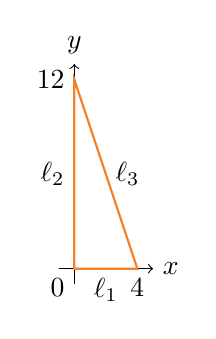
\begin{tikzpicture}[scale=0.20]
                  \draw[->] (-1,0) -- (5,0) node[right] {\(x\)};
                  \draw[->] (0,-1) -- (0,13) node[above] {\(y\)};
                  \draw[color=horange, thick] (0,0) -- (4,0) -- (0,12) -- cycle;
                  \node[below left] at (0,0) {\(0\)};
                  \node[below] at (4,0) {\(4\)};
                  \node[left] at (0,12) {\(12\)};
                  \node[below] at (2,0) {\(\ell_{1}\)};
                  \node[left] at (0,6) {\(\ell_{2}\)};
                  \node[right] at (2,6) {\(\ell_{3}\)};
                \end{tikzpicture}
              \end{minipage}%
              \begin{minipage}{0.3\textwidth}
                \begin{align*}
                  \ell_{1} & : y = 0 \\
                  \ell_{2} & : x = 0 \\
                  \ell_{3} & : y = -3x + 12
                \end{align*}
              \end{minipage}
            \end{center}
            

            This gives us the limits of integration as follows:
            \[
              \{(x,y) \colon 0 \leq x \leq 4, \quad 0 \leq y \leq -3x + 12\}.
            \]
            Thus, we can write the double integral as:
            \begin{align*}
              \iint_{D}(x^{2} + 6xy) \, dA & = \int_{0}^{4}\int_{0}^{-3x + 12}(x^{2} + 6xy) \, dy \, dx \\
              & = \int_{0}^{4}\left[x^{2}y + 3xy^{2}\right]_{0}^{-3x + 12} \, dx \\
              &= \int_{0}^{4}\left[x^{2}(-3x + 12) + 3x(-3x + 12)^{2}\right] \, dx \\
              &= \int_{0}^{4}\left[-3x^{3} + 12x^{2} + 3x(9x^{2} -72x + 144)\right] \, dx \\
              &= \int_{0}^{4}\left[24x^{3} - 204x^{2} + 432x\right] \, dx \\
              &= 6 \int_{0}^{4}\left[4x^{3} - 34x^{2} + 72x\right] \, dx \\
              &= 6\left[x^{4} - \tfrac{34}{3}x^{3} + 36x^{2}\right]_{0}^{4} \\
              &= 48\left[32 - \tfrac{34}{3}(8) + 36(2)\right] \\
              &= \boxed{640}
            \end{align*}
          }
          \item \(\displaystyle\int_{0}^{2}\int_{x^{2}}^{4} 4x^{3}\cos(y^{3}) \,dy\,dx\) \\

          \sol{
            To evaluate this integral, we must change the order of integration. The original region is:
            \[
              \{(x,y) \colon 0 \leq x \leq 2, \quad x^{2} \leq y \leq 4\}.
            \]
            The new region is:
            \[
              \{(x,y) \colon 0 \leq y \leq 4, \quad 0 \leq x \leq \mysqrt{y}\}.
            \]
            Thus, we can rewrite and solve the double integral:
            \begin{align*}
              \int_{0}^{2}\int_{x^{2}}^{4} 4x^{3}\cos(y^{3}) \,dy\,dx & = \int_{0}^{4}\int_{0}^{\mysqrt{y}} 4x^{3}\cos(y^{3}) \,dx\,dy \\
              & = \int_{0}^{4}\left[ x^{4}\cos(y^{3})\right]_{0}^{\mysqrt{y}} \,dy \\
              & = \int_{0}^{4}y^{2}\cos(y^{3}) \,dy \\
              & = \left[\tfrac{1}{3}\sin(y^{3})\right]_{0}^{4} \\
              & = \tfrac{1}{3}\left[\sin(64) - 0\right] \\
              & = \boxed{\tfrac{1}{3}\sin(64)}.
            \end{align*}
          }
          \textit{No problems like this where we have to switch the order of integration on the exam.}
  %         \item \(\displaystyle\int_{-3}^{3}\int_{0}^{\mysqrt{9-x^{2}}} \sin(5x^{2} + 5y^{2}) \,dy\,dx\) \\

  %         \sol{
  %           We again must change the order of integration for this integral. First, we know the original region is:
  %           \[
  %             \left\{(x,y) \colon -3 \leq x \leq 3, \quad 0 \leq y \leq \mysqrt{9 - x^{2}}\right\},
  %           \]
  %           which is the upper half of the disk \(x^{2} + y^{2} \leq 9\). Hence, we should write the coordinates in polar form:
  %           \[
  %             x = r \cos(\theta), \quad y = r \sin(\theta), \quad \text{and} \quad dx \, dy = r \, dr \, d\theta.
  %           \]
  %           Since \(y \geq 0\), the angle \(\theta\) must be between \(0\) and \(\pi\) and \(r\) is between \(0\) and \(3\). In addition, we can make our equation of the integrand simpler:
  %           \[
  %             \sin(5x^{2} + 5y^{2}) = \sin\Big(5r^{2}\big(\cos^{2}(\theta) + \sin^{2}(\theta)\big)\Big) = \sin(5r^{2}).
  %           \]
  %           Now we can solve the integral:
  %           \begin{align*}
  %             \int_{0}^{\pi}\int_{0}^{3} \sin(5r^{2}) r \, dr \, d\theta & = \int_{0}^{\pi} d\theta \cdot \left[-\tfrac{1}{10}\cos(5r^{2})\right]_{0}^{3} \\              
  %             & = \left[-\tfrac{1}{10}\cos(45) + \tfrac{1}{10}\cos(0)\right] \\
  %             & = -\tfrac{1}{10}\left(\tfrac{\mysqrt{2}}{2} - 1\right) \\
  %             & = -\tfrac{1}{20}\left(\mysqrt{2} - 2\right) \\
  %             & = \boxed{-\tfrac{\mysqrt{2}}{20} + \tfrac{1}{10}}.
  %           \end{align*}
  %         }
  %         \item \(\displaystyle\int_{0}^{1}\int_{0}^{\mysqrt{1-x}}\int_{0}^{\mysqrt{1-x^{2}-y^{2}}} \mysqrt{x^{2} + y^{2} + z^{2}} \,dz\,dy\,dx\) \\
          
  %         \sol{
              \textit{Convert to spherical coordinates. Gives}
  %         }
        \end{enumerate}
  % \item (3 points) Find the volume of the solid described by \(x^{2} + y^{2} \leq 1, \quad x \geq 0, \quad 0 \leq z \leq 4 - y\). \\

  % \sol{

  % }
  % \item (3 points) Find the average value of the function \(f(x,y) = x\sin(y)\) over the region enclosed by \(y = 0\), \(y = x^{2}\), and \(x = 1\). \\

  % \sol{

  % }
  % \item (3 points) Find the volume of the solid that lives within both the cylinder \(x^{2} + y^{2} = 1\) and sphere \(x^{2} + y^{2} + z^{2} = 9\). \\
  
  %       \sol{
  %         Use cylindrical coordinates.
  %       }
\end{enumerate}
\vspace{2cm}
\begin{center}
\textsc{REST ON PAPER}
\end{center}

Find the value of \(\iint_{D}x^{2}y \, dA\) where \(D\) is the region between the \(x\)-axis and the upper semicircle\(y = \sqrt{9 - x^{2}}\).

and 

Let \(E\) be the part of the unit sphere which lives in the first octant. Determine the exact value of \(\iiint_{E}(x^{2}z + y^{2}z + z^{3})\, dV\).

and

Consider the cylinder, with central axis along the \(y\)-axis, of radius 3 between the \(xy\)-plane and the plane \(y = 10\). The temperature, \(T\), at any point inside the cylinder is given by \(T(x,y,z) = x^{2}yz^{2}\). Determine the average temperature inside the cylinder. 


\end{document}
